% This is the project description we were provided we can tailor it later

\begin{itemize}
\item \textbf{Physical Structure} 

$\indent$ Silicate glasses are very important materials in fields including medicine, optics, electronics, telecommunication and energy. Typically in these silicate glasses there exists a structure where silicon (Si) is surrounded by four oxygen (O) atoms forming a tetrahedron seen in Figure 1. These tetrahedra share one common O atom if they are neighbors. A ring forms if a group of tetrahedra share common O atoms, and the size of these rings is computed based on how many Si atoms are in the ring. A large ring has 11 and 12 Si atoms, medium rings have 5 and 6, and small rings have 1 or 2. An atom is denoted as under-coordinated if the number of its constraints is lower than 4, and over-constrained, if greater than 4. \cite{pedone2015dynamics}
\begin{figure}
    \centering
    \noindent
    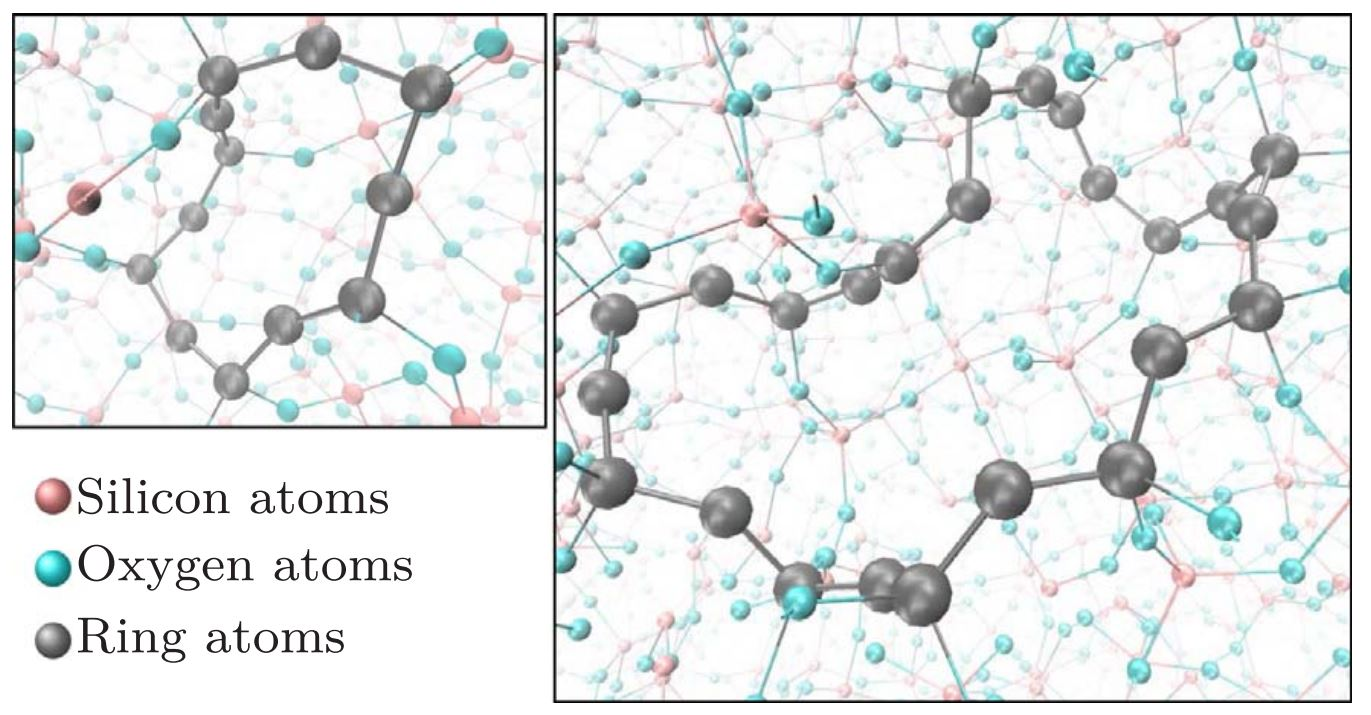
\includegraphics[width=12cm, height=6cm]{picture/tetra.JPG}
    \caption{Example of a primitive sixfold ring (left), example of a primitive twelve-fold ring
(right) \cite{ebrahem2018influence}}
    \label{crack_Fig}
\end{figure}
\end{itemize}


\begin{itemize}
\item \textbf{Molecular Dynamics Simulations} 

Classical molecular dynamics simulations were also used to investigate the properties of silicate glasses. One particular simulation of interest is of crack propagation at the atomic level. Figure \ref{crack_prop} shows a 3D visualization of this simulation with perspective. Given that glass is extremely brittle, fractures may occur instantaneously when a maximum stress level is reached.
\bigskip
%%  CRACK PROPEGATION SIMULATION FIGURE 
\begin{figure}
    \centering
    \noindent
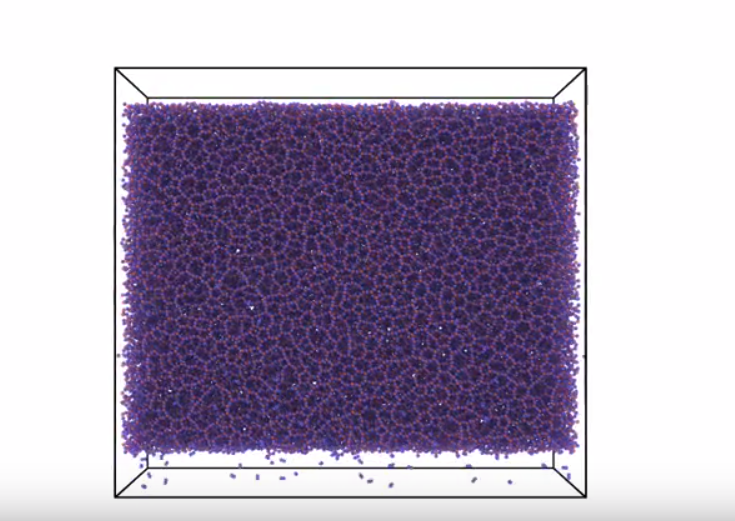
\includegraphics[width=0.4\textwidth]{picture/frac_prop1.PNG}\hspace{0.2\textwidth}%
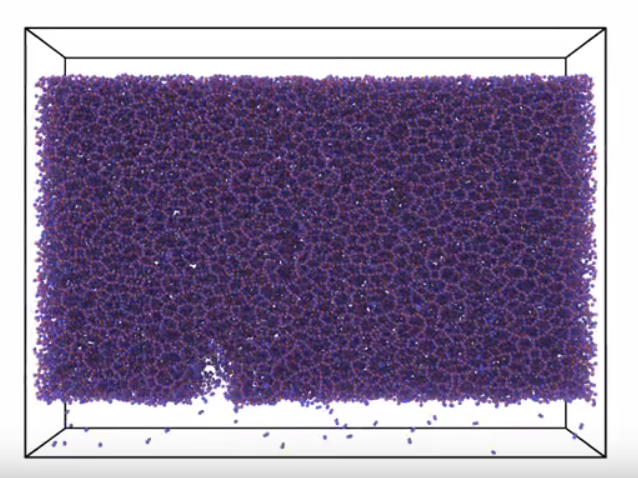
\includegraphics[width=0.4\textwidth]{picture/frac_prop2.PNG}\\[2em]
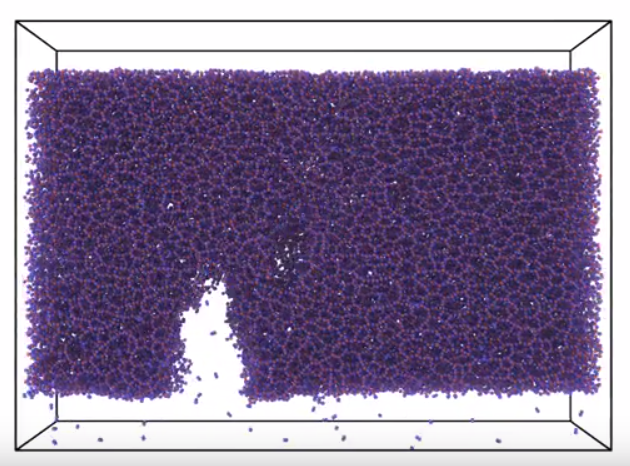
\includegraphics[width=0.4\textwidth]{picture/frac_prop3.PNG}\hspace{0.2\textwidth}%
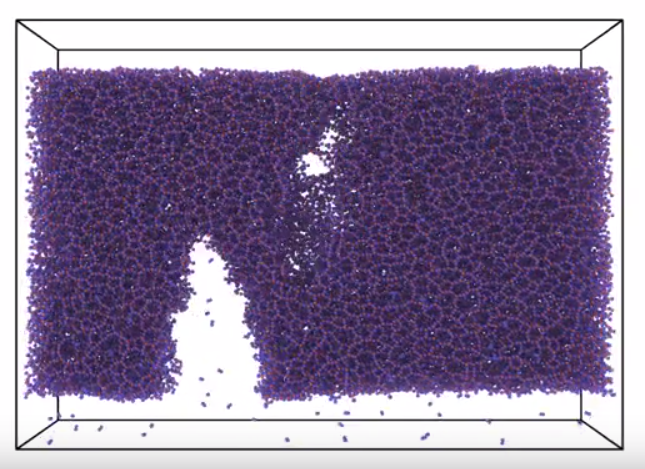
\includegraphics[width=0.4\textwidth]{picture/frac_prop4.PNG}\par
    \caption{Crack propagation in MD simulations.}
    \label{crack_prop}
\end{figure}
%%%%%%%%%%%%%%%%%%%%%%%%%%%%%%%%%%%%%%% Glasses were observed using 60k atoms for soda-silicate glasses and 30k atoms for silica glass . Soda-lime silicate glasses were analyzed at the nanometric scale with an atomic force microscope. Cavities were formed at 20nm long and 5nm deep ahead of the crack tip, and cracks would advance following the coalescence of cavities .

Regarding the mechanical properties of the silicate glass, Young's modulus, strength, failure strain and fracture mechanism were all used throughout the study.  Additionally, these properties depend on both the strain rate and the quench rate. The glasses were heated at 5000 K, a temperature considered more than adequate to bring the glass into a liquid state and the heat was equilibrated for 100 picoseconds and then cooled continuously to 300 K with a normal cooling rate of 5 K/ps.

It is also shown that when the quench rate increases there was an increase in the number of large-sized rings and a decrease in the number of medium-sized rings. The change in the number of small-sized rings was minimal. Since there is larger void in large-sized ring, it can be stretched and deformed more than the medium-sized ring. However, a medium-sized ring can take more per unit stress while tensile is applied, so it has more strain energy \cite{mWilson_continuum_stress}.

With regards to stress, uni-axial tensile tests were implemented along the z-axis for both bulk glasses and nanowires. An important finding is such that for uni-axial tension tests in bulk glasses, in particular flaw-free silica glass, the glass was forced to break in a brittle manner. Additionally, in flaw-free glass, voids would grow, then coalesce before the structure would fracture. What was concluded as a result of the numerous tests performed was that the fracture mechanism of defective models showed to be less brittle compared to flaw-free glass given the unstable region is capable of expansion.\cite{radialDistribution}.
\end{itemize}

\begin{itemize}
\item \textbf{Motivation} 

$\indent$ Nucleation of fractures originates from defects of the atomic structure of silicate glass. 
The fractures do not necessarily occur when the weakest bond in the structure breaks and triggers numerous other breaks in the surrounding bonds. Instead, the fracturing is dependent on the local structure surrounding the atoms so defining this relation is critical in the fracture analysis. While these relations can be studied using results from MD, a repetitive simulation-observation approach is computationally prohibitive. A more tractable approach is to use machine learning and surrogate modeling techniques \cite{TopSystem} \cite{MLACrack} \cite{bauchy}. 

Molecular dynamics (MD) simulations have shown that silicates that have their fracture regions contacted with an aqueous environment have their Si-O bond energy threshold lowered by 25$\%$  \cite{chem_effects}. Since there is both mechanical loading (stress) and chemical that affect the crack tips, it becomes more difficult to predict fracture propagation. Running simulations of the chemical-mechanical effects on crack tips showed differing rates of fracture propagation as well as changes in fracture direction and even stress distribution in the atoms in the fracture process zone. 

Therefore, knowing the initial conditions of the silicate glass environment is critical in predicting fracture behavior and  will test the robustness of our model.
\end{itemize}


\begin{itemize}
\item \textbf{Data} 

$\indent$ Sandia National Labs will provide the MD simulation data used for training the surrogate model. At the present time 100 simulations have been constructed each consisting a sample of a fracture at the atomic level. The training data is broken up into the following four parts:

\begin{enumerate}
    \item Dry (vacuum), free surfaces on the y,z axis and periodic in the x direction.
    \item Wet (H20 in interstices), free surfaces as above. 
    \item Dry (vacuum), fully periodic (toroidal) in x,y and z axis.
    \item Wet (H20 in interstices), fully periodic (toroidal) boundary conditions. 
\end{enumerate}

For each sample, uniaxel tension is performed until failure or up to .5 starin over 1\textit{ns} simulation time. 

The silicate is exposed to these conditions following uniform quenching process done at 3.7K/picoseconds. The quenching process is controlled in order to limit the variance in the arrangement of the tetrahedra structure \cite{ebrahem2018influence}. We have four different environmental conditions but all procedures start at equilibrium.
Each instance will contain snapshots ($\Delta$ t = 1\textit{ps} ) of the atoms through time as well as information regarding charge, stress tensor and bond connectivity. \cite{markpres}

Post processed data was also provided as well as Python scripts to create and modify simulation data. 

\end{itemize}






%% ANOTHER PICTURE 
%\begin{figure}[!b]
%  \centering
%  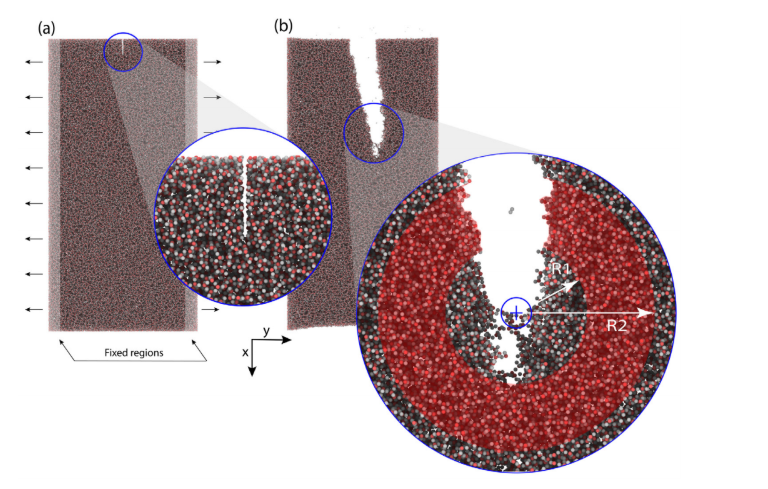
\includegraphics[width=11cm]{picture/FractureMechanism.PNG}
%  \caption{Images of a simulated a-SiO2 sample. (a) Samples are loaded and held in mode I tension. Initial %cracks are created by removing a
%small number of atoms from the upper surface of the sample. (b) An example of crack propagation in a %loaded sample, with the crack tip
%identified by the +, and the annulus colored red. Figure reproduced %from~\protect\cite{mWilson_continuum_stress}} 
%  \label{crack_prop2}
%\end{figure}


%% EL NUMERO TRES 
%\begin{figure}[!h]
%  \centering
%  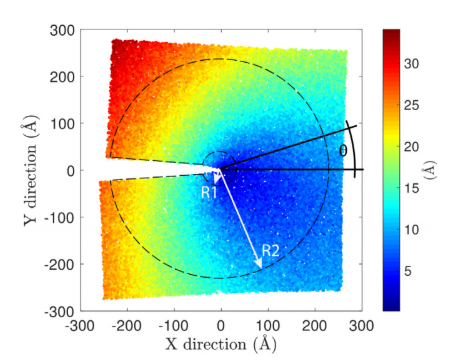
\includegraphics[width=11cm]{picture/FractureMechanism2.PNG}
%  \caption{Configuration showing the coordinate axes and crack tip relationship similar to the Williams %expansion. Dashed lines show an annulus
%with inner radius R1 and outer R2. Points are colored according to the magnitude of their displacement %%under an applied field. Figure reproduced from~\protect\cite{mWilson_continuum_stress}} 
 % \label{crack_rad2}
%\end{figure}